%!TEX root = ./lec03_hardware.tex


%
% ---------------------------------------------------------------------------
%
\begin{frame}
\label{architecture}

Virtually all computers today, from cell phones to servers, have the same internal architecture, introduced by John Von Neumann in the 1945\footnote{\url{https://en.wikipedia.org/wiki/Von_Neumann_architecture}}.

\vskip1em

\begin{columns}[onlytextwidth]
\begin{column}{0.4\textwidth}
Both programs and data are \textbf{stored in memory}.\\[1em]
Programs are executed by the Central Processing Unit (CPU), one instruction at a time.\\[1em]
Constant move of code and data between memory and CPU.
\end{column}
\begin{column}{0.6\textwidth}
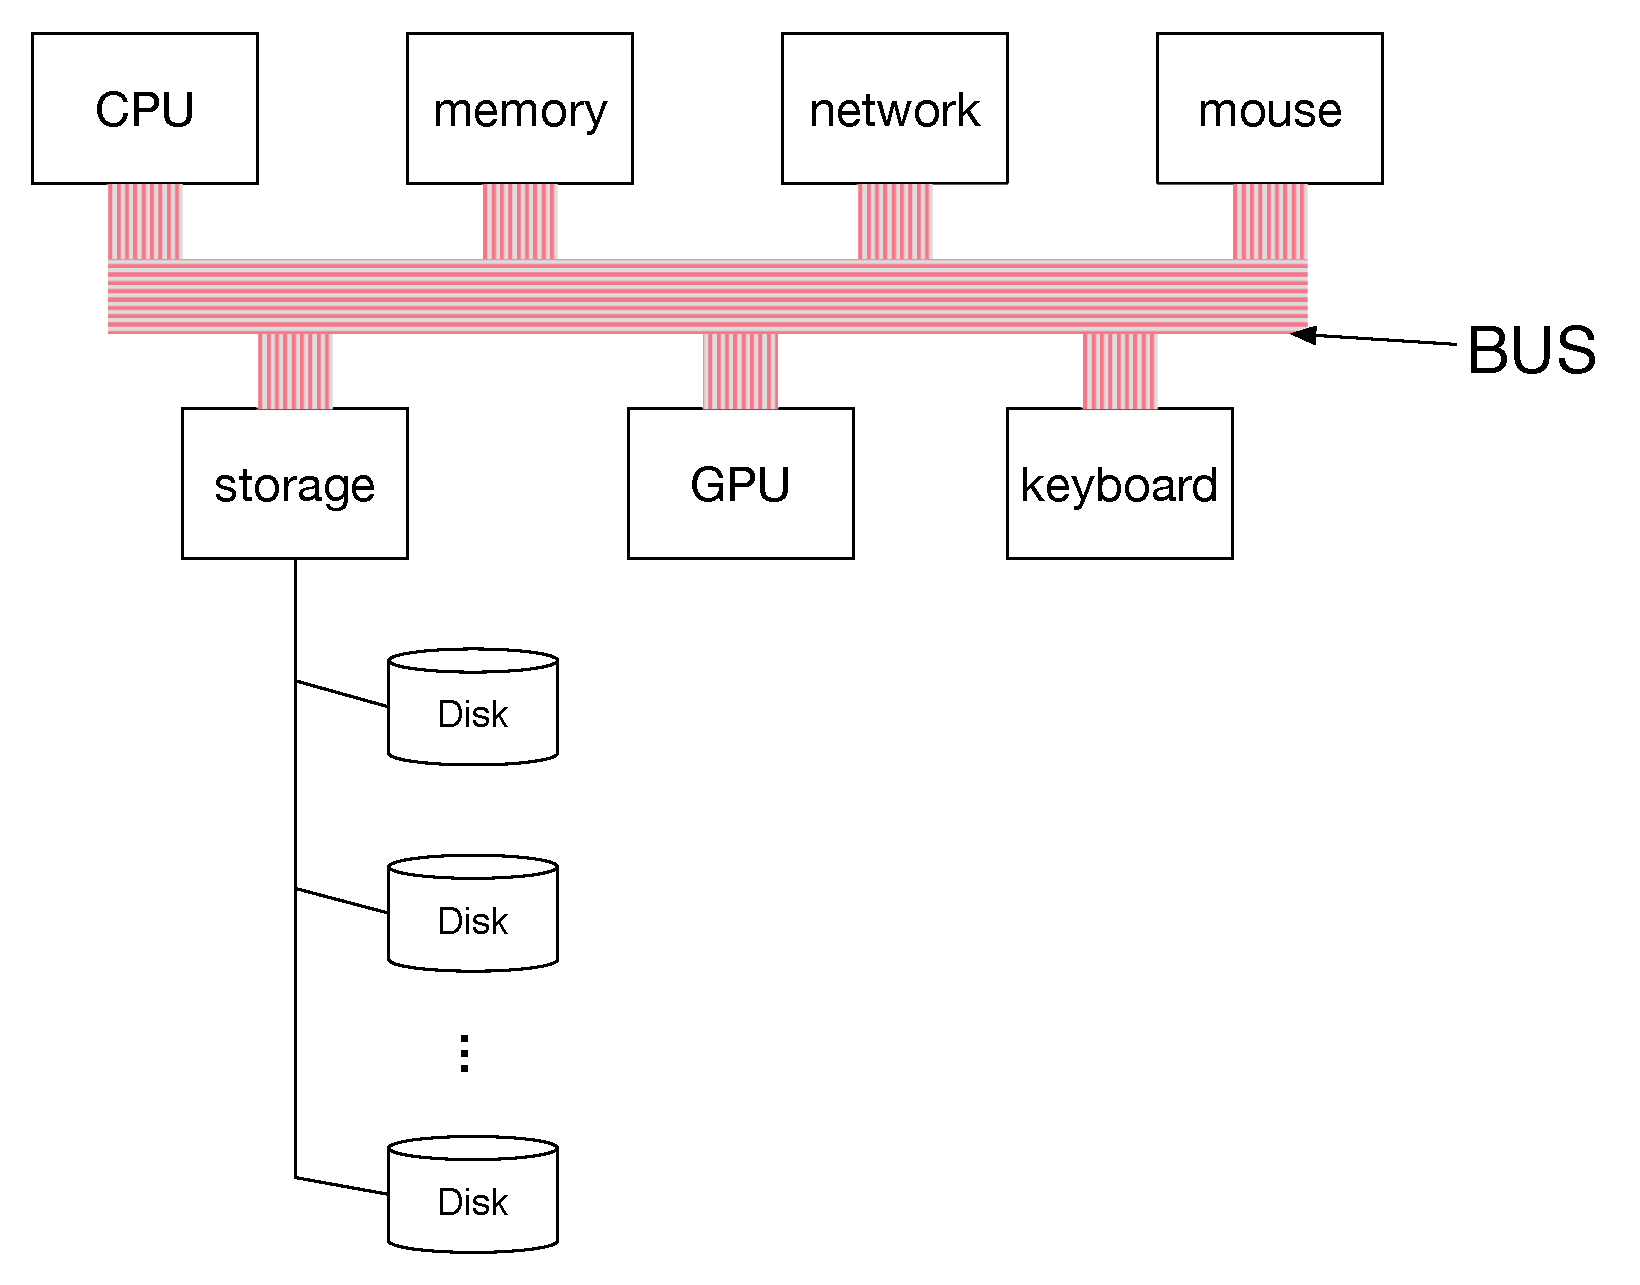
\includegraphics[width=1.1\textwidth]{./figures/von_neumann_architecture}
\end{column}
\end{columns}
\end{frame}

\begin{frame}

Components are interconnected by a Bus\footnote{\url{https://en.wikipedia.org/wiki/Bus_(computing)}}.

\begin{center}
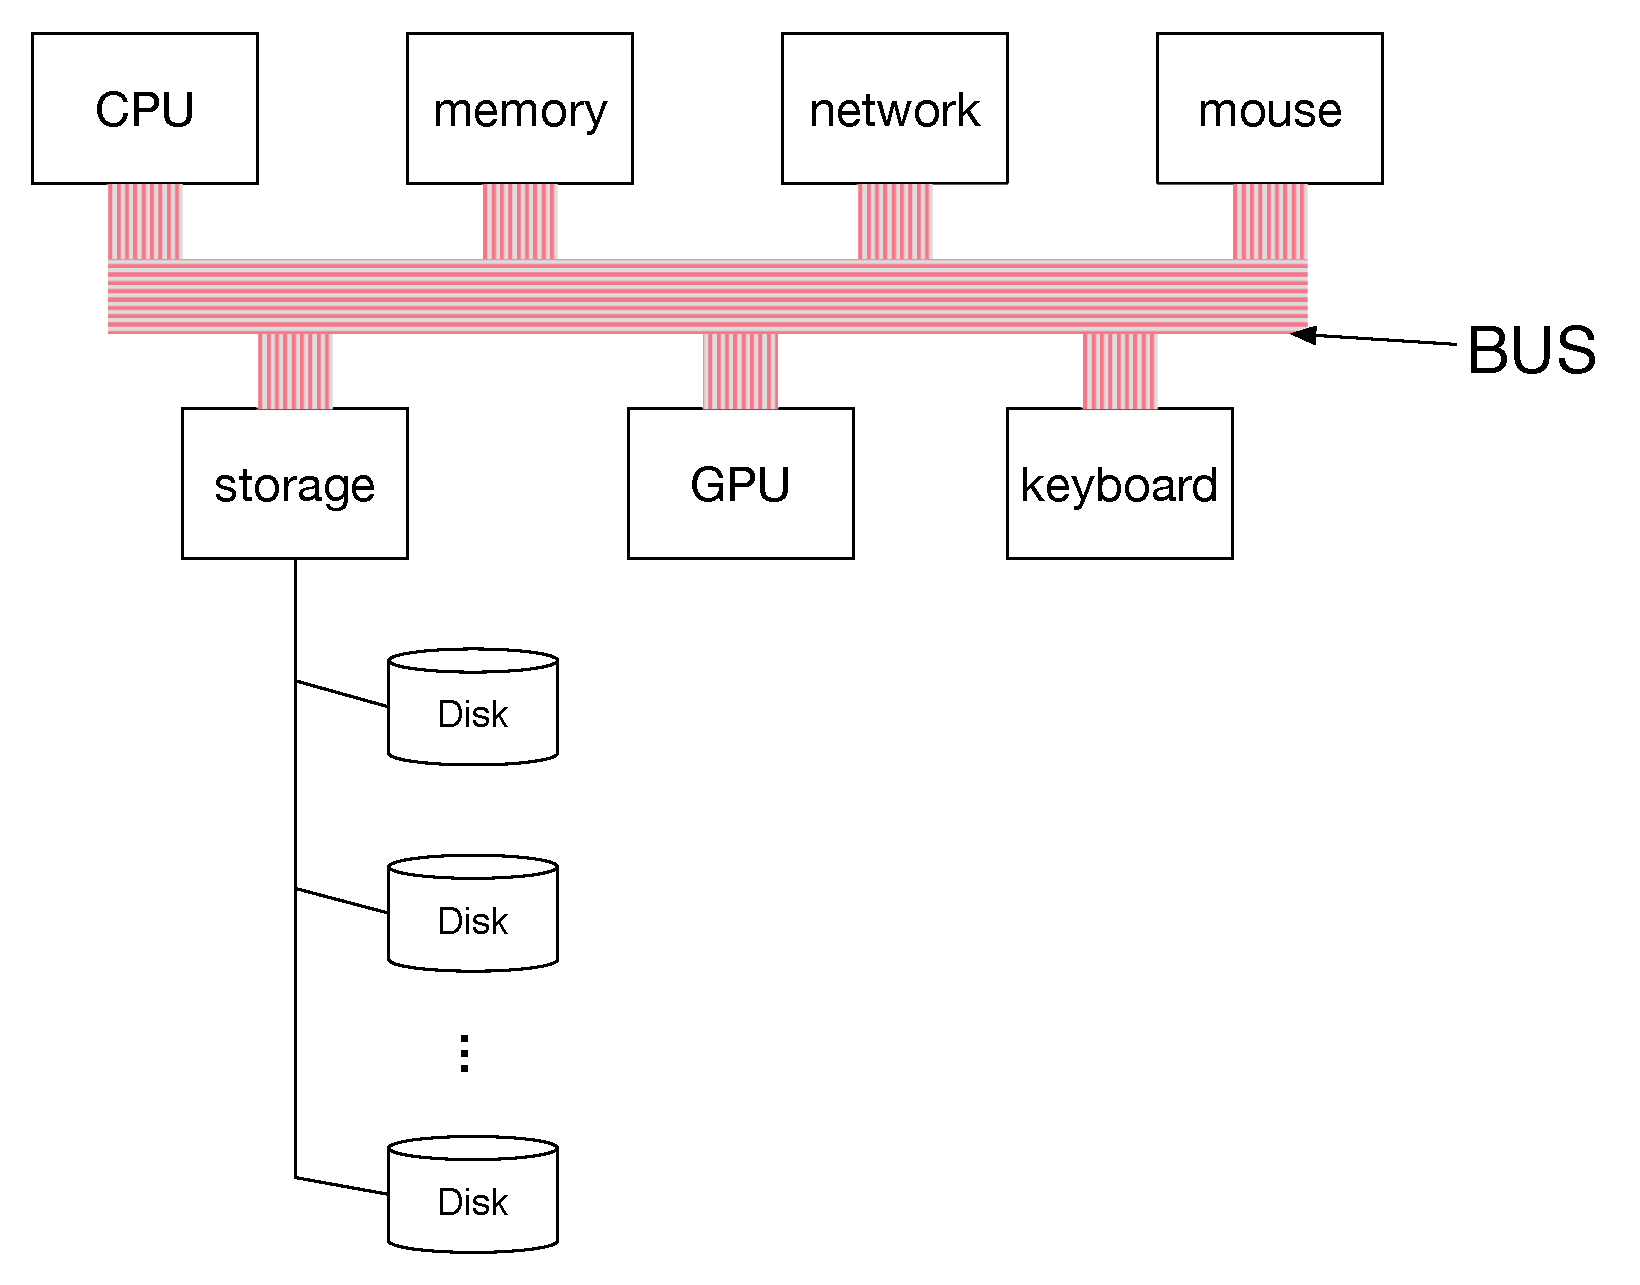
\includegraphics[trim={0 12cm 0 0},clip,width=0.65\textwidth]{./figures/von_neumann_architecture}
\end{center}

\vskip1em 

\begin{block}{The BUS \alert{must be \textbf{shared} by} all components.}
It can only be used for \textbf{unidirectional} transfers between two components at a time (e.g., from memory to the CPU).
\end{block}

% \vskip0.25em 

To maximize efficiency, transfers between \textbf{storage and memory} or \textbf{memory and CPU} are made in \alert{\textbf{fixed-sized batches}} (called \alert{memory pages} or \alert{disk blocks}).

\vskip1em 

\end{frame}

\begin{frame}

As far as the DBMS is concerned, these three components are the most important:

\begin{center}
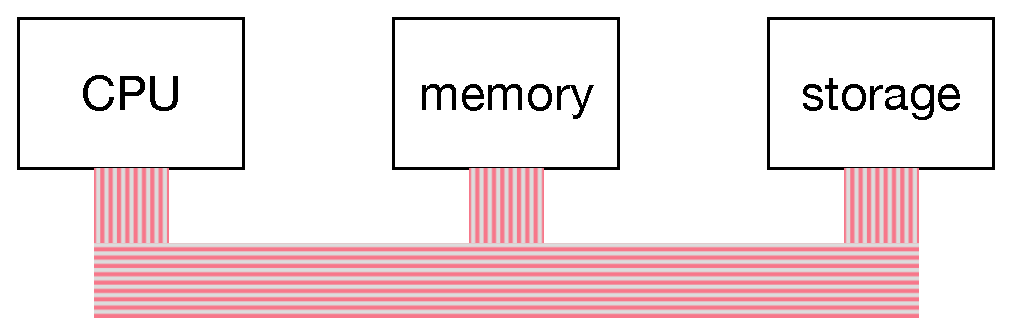
\includegraphics[width=0.5\textwidth]{figures/von_neumann_architecture_2}
\end{center}

The CPU is where the DMBS code runs (e.g., where SQL queries are executed).

The storage is where the database is stored persistently (i.e., even when the computer is off).

Memory is where the data from storage resides before it can be used by the CPU.

\end{frame}


\begin{frame}

However, the CPU does not access data in storage directly. 

\textbf{Memory-mapped I/O:} access to data on files is done by mapping those files to buffers in memory.

\vskip2em

\begin{center}
\includegraphics[width=0.5\textwidth]{figures/memory_mapped_io}
\end{center}

\vskip1em

The memory is at the center of modern architectures, so we will look at how it works first.

\end{frame}


\begin{frame}

Memory is organized as a grid of cells, each with a \underline{unique address}. 

The number of addresses depends on the computer. Typically, 32-bit computers have $2^{32}$ addresses, 64-bit computers have $2^{64}$ addresses, and so on.

\vskip1em

\begin{columns}[onlytextwidth]
\begin{column}{0.225\textwidth}
Ex: computer with \textbf{6-bit} addresses, for a memory with $2^6=64$ cells.

\vskip1em

Each cell holds a fixed-sized \textbf{word} (typically 64 bits).

\vskip1em

~
\end{column}
\begin{column}{0.75\textwidth}
\hspace*{2em}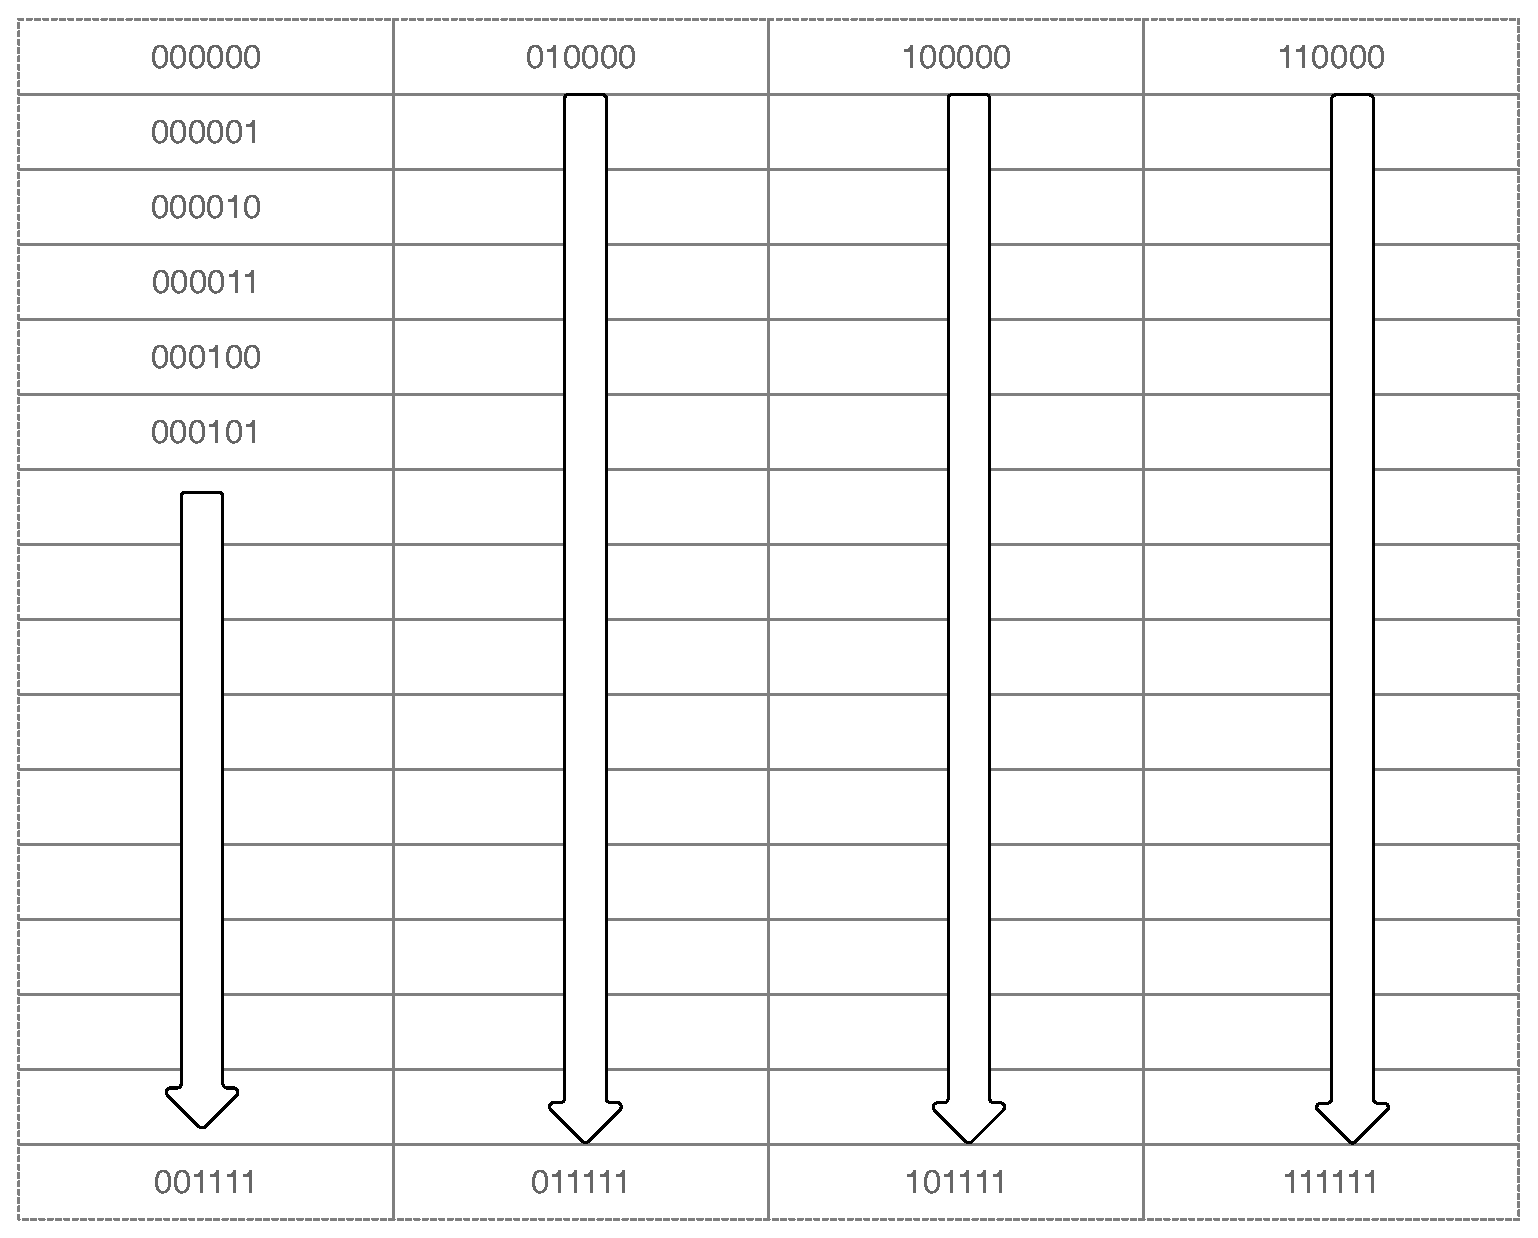
\includegraphics[width=0.9\textwidth]{figures/64_cell_memory_diagram}
\end{column}
\end{columns}
\end{frame}



\begin{frame}

The bits in the memory address are divided into two parts. Some bits are used to indicate a \textbf{page of memory}, and the other bits are used to indicate an \textbf{offset} inside the page.

\vskip1em

\begin{columns}[onlytextwidth]
\begin{column}{0.225\textwidth}
Ex: \alert{4} bits for a \alert{page} and \blue{2} bits for the \blue{offset}.

\vskip1em

So, the memory in our example is divided into $2^{\alert{4}}= \alert{16}$ pages, each with $2^{\blue{2}}=\blue{4}$ cells.
\vskip1em


\end{column}
\begin{column}{0.75\textwidth}

\begin{tikzpicture}
\node at (0,0) [anchor=south west] {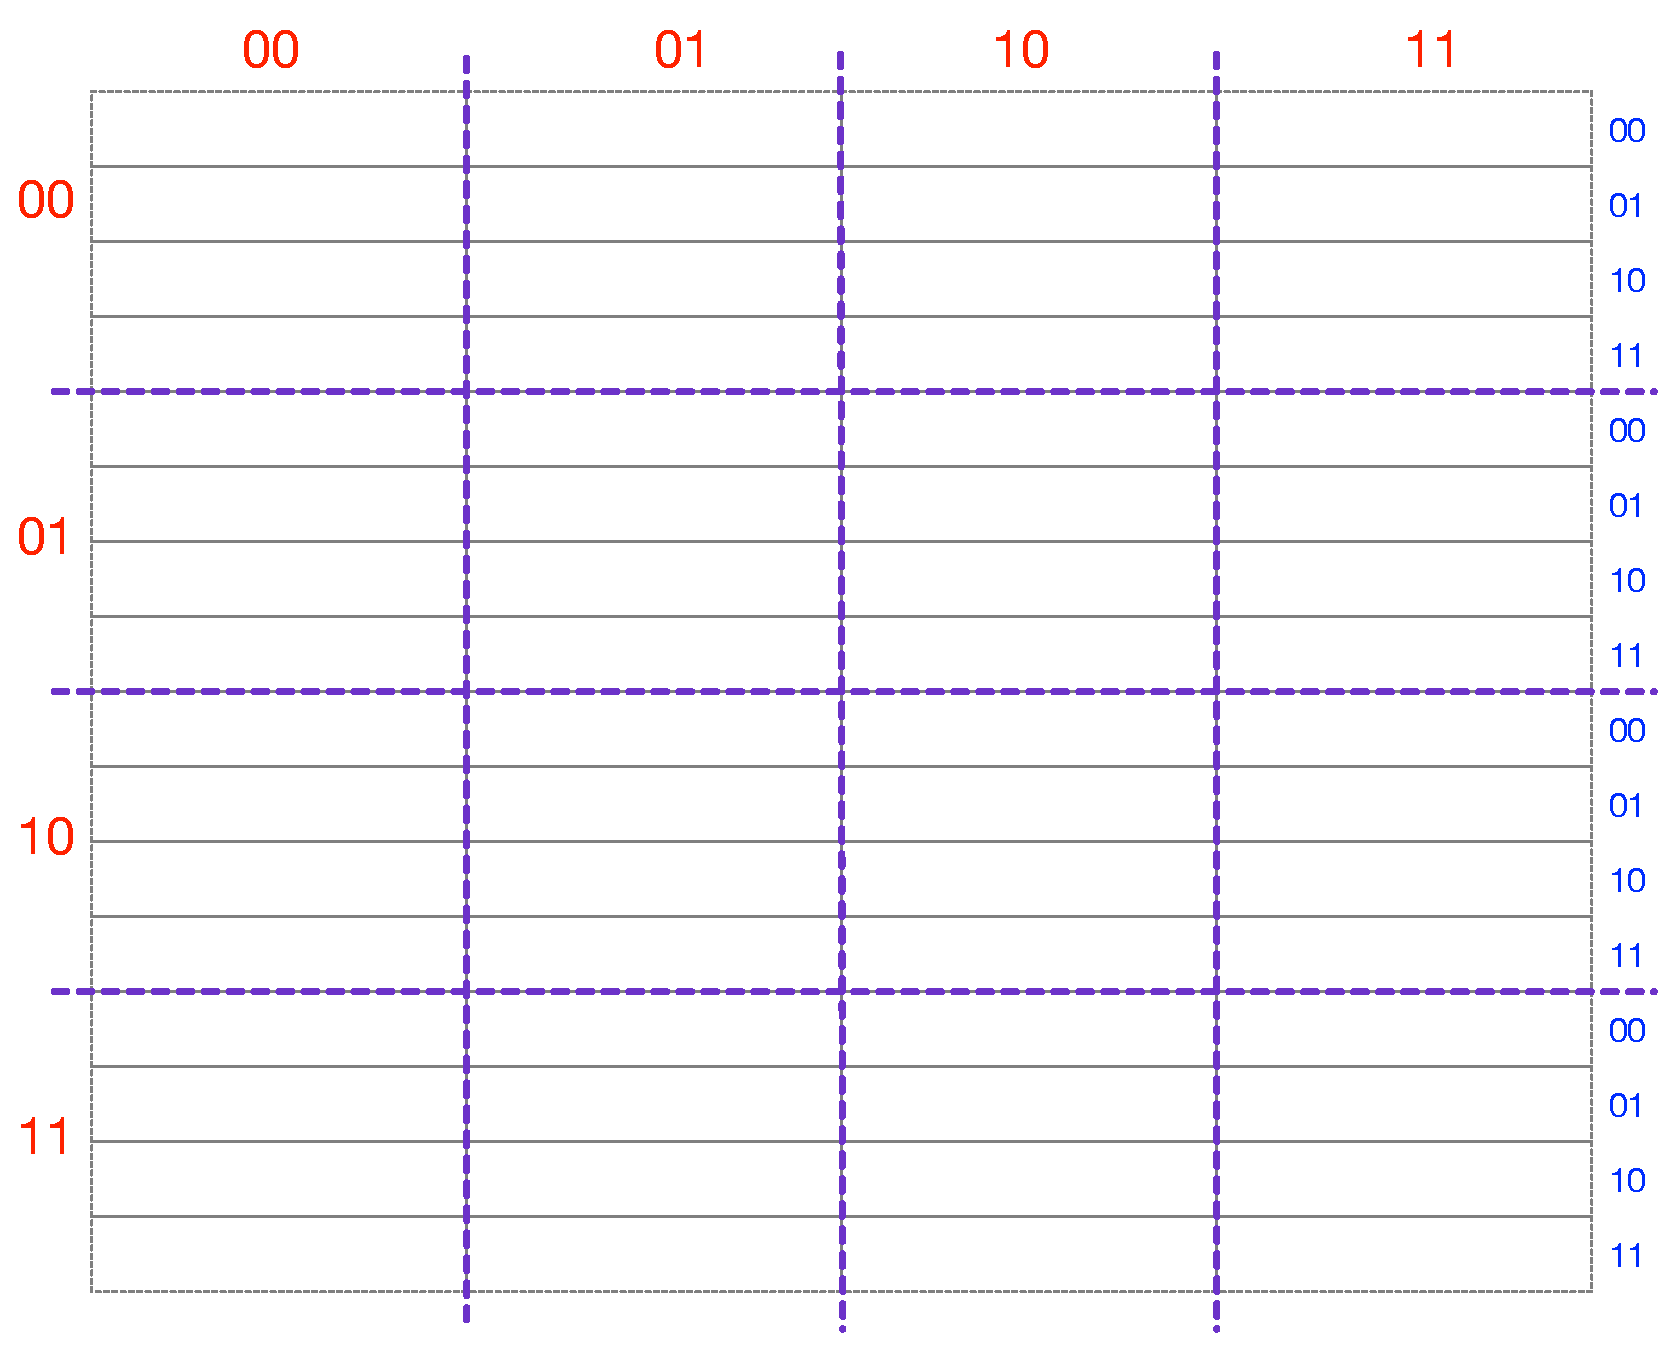
\includegraphics[width=\textwidth]{figures/6_bit_memory_grid}};
\draw[draw=red,line width=1.5pt] (4.2,3.3) rectangle ++(1.85,1.45) 
	node [fill,anchor=north east,yshift=10pt,xshift=-10pt,text=red,fill=white] {page};
\end{tikzpicture}

\end{column}
\end{columns}
\end{frame}

\newsavebox\CExample
\begin{lrbox}{\CExample}
\begin{lstlisting}[style=C]

data = (int*) malloc(20 * sizeof(int));

// initialize data array...

for (int i = 0; i < 20; i++){
    data[i] = data[i] + 1;
}
\end{lstlisting}
\end{lrbox}



\begin{frame}[fragile]

Consider a hypothetical C program:

\begin{center}
\framebox{\scalebox{0.75}{\usebox{\CExample}}}
\end{center}

The program is compiled into binary code and stored into one or more disk blocks. When the program is \underline{executed}, each block is brought to a \underline{page in memory}.

Dynamically allocated data structures are stored on (possibly many) pages in memory as well.

The local variable \lstinline[style=C]!data! is represented in the program \emph{heap} and contain the address in memory where the actual array is located.

\end{frame}


%
% ---------------------------------------------------------------------------

\newsavebox{\MemoryPagesBox}
\savebox{\MemoryPagesBox}{
	\hspace*{-1em}\begin{tikzpicture}
\node at (0,0) [anchor=south west] {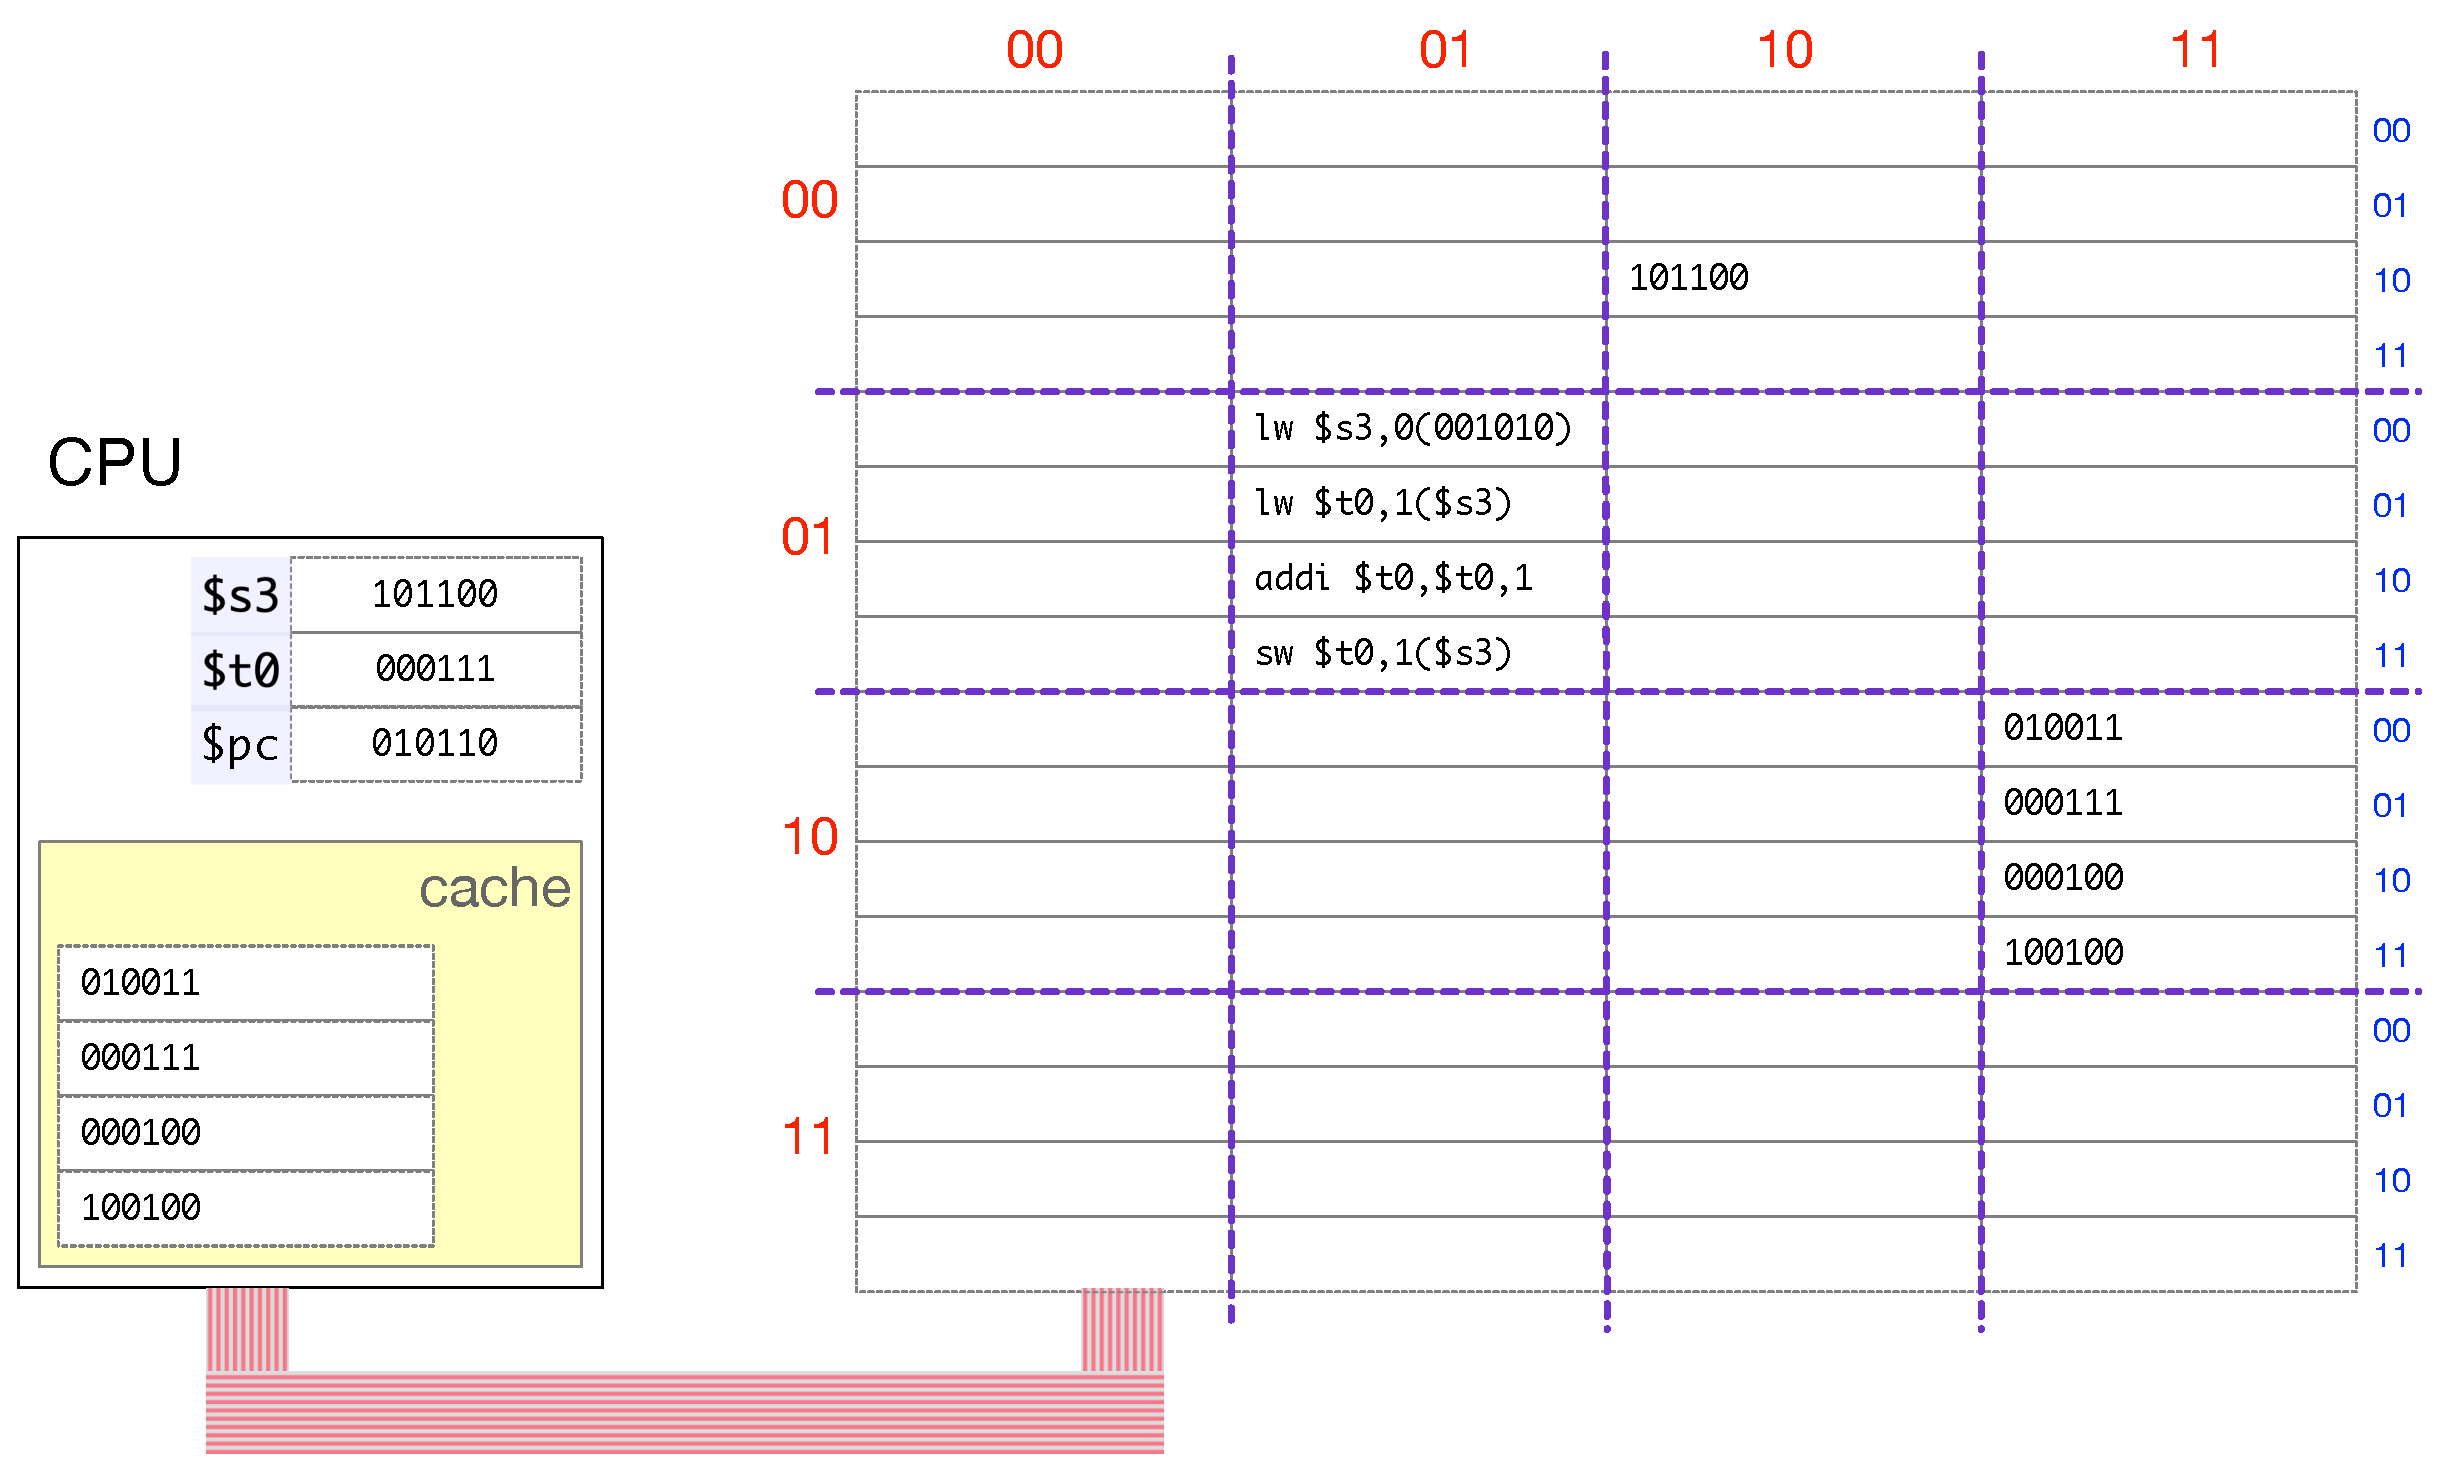
\includegraphics[width=1.2\textwidth]{./figures/CPU_memory_detailed}};
\only<1>\draw[draw=red,line width=1.5pt] (6.7,4.25) rectangle ++(2,1.6) 
	node [fill,anchor=north east,yshift=10pt,xshift=-5pt,text=red,fill=white] {program};
\only<2>\draw[draw=red,line width=1.5pt] (8.7,5.9) rectangle ++(2,1.6) 
	node [fill,anchor=north east,yshift=10pt,xshift=-12pt,text=red,fill=white] {heap};	
\only<3>\draw[draw=red,line width=1.5pt] (10.7,2.6) rectangle ++(2,1.6) 
	node [fill,anchor=north east,yshift=10pt,xshift=-12pt,text=red,fill=white] {data};
\end{tikzpicture}
}
%
\begin{frame}
\vskip1em

\begin{center}
\scalebox{0.75}{\usebox{\MemoryPagesBox}}
\end{center}

Even though the memory sends entire pages to the CPU, the \underline{program instructions use individual memory cells}.

A cache memory inside the CPU holds copies of pages in memory, from where the CPU can access the cells.

\end{frame}

%
% ---------------------------------------------------------------------------
%
\begin{frame}{The CPU}

The CPU works in \textbf{cycles}, defined by internal ticking \alert{clock} (1 GHz = 1 billion ticks per second).

Abstractly speaking, in each cycle, the CPU:\\
(1) fetches the \textbf{next}\footnote{The \textbf{program counter} (\lstinline{$pc}) register keeps the address of that instruction.} instruction of the program, \alert{from memory}\\
(2) decodes and executes the instruction \\
(3) increments the program counter to the next instruction

\begin{BOX}{Program vs CPU instructions}
Each instruction in a program in a high-level language (e.g., a \lstinline[style=C]{printf()} statement) gets compiled into many (sometimes thousands) of CPU instructions.
\end{BOX}


\end{frame}

%
% ---------------------------------------------------------------------------
%
\begin{frame}

The registers (e.g., \alert{\$s3}, \alert{\$pc}) are circuits inside the CPU that can hold the content of a \textbf{single word} in memory.

\vskip0.5em

Arithmetic (and other) operations values stored in registers:\\
 - ex: \alert{\lstinline[style=C]!addi $t0,$t0,1!} adds a constant (1) to the value in register \lstinline[style=C]{$t0}\\
 - the results of these operations are written back to registers.

\vskip1em

\begin{BOX}{The CPU \textbf{does not manipulate} memory cells directly }
instead it must move data from memory into registers (via the cache memory) and back:\\
 - ex: \textbf{load a word from memory}: \lstinline[style=cmput391]{-:lw :- <register>,<address>}\\
 - ex: \textbf{store a word into memory} : \lstinline[style=cmput391]{-:sw :- <register>, <address>}
\end{BOX}
\end{frame}


% ---------------------------------------------------------------------------

\begin{frame}{Multi-core CPUs}

Modern CPUs have many (typically, between 2 and 32) independent processors (or \textbf{cores}).

\vskip1em

\begin{columns}[onlytextwidth]
\begin{column}{0.45\textwidth}
Each core has its own private (L2) cache, but can also use a larger shared (L3) cache.

\vskip1em

Multiple programs can run at the same time, on different cores.
\end{column}
\begin{column}{0.5\textwidth}
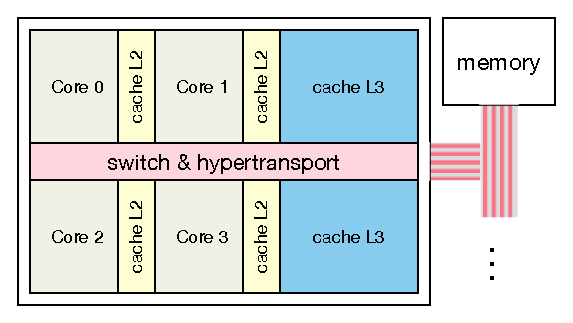
\includegraphics[width=1.1\textwidth]{figures/multicoreCPU.eps}
\end{column}
\end{columns}

\vskip0.5em

Moreover, the same program can be broken into multiple processes (also called \emph{threads}) which can run \textbf{at the same time} on different cores.

\end{frame}


%
% ---------------------------------------------------------------------------
%
\begin{frame}{Volatile and persistent memory}

\begin{columns}[onlytextwidth]
\begin{column}{0.475\textwidth}
\begin{BOX}{Volatile Memory}
Memory that needs continuous power to keep its contents. Also called \emph{transient} memory.\\[1em]
Ex: registers, caches, \alert{RAM}
\end{BOX}
\end{column}
\begin{column}{0.475\textwidth}
\begin{BOX}{Persistent Memory}
Memory that keeps its contents even without continuous power.\\ \alert{Also known as \emph{storage}}.\\[1em]
Ex: HDDs and SSDs
\end{BOX}
\end{column}
\end{columns}

\vskip1em

The \alert{``main memory''} refers to RAM (Random Access Memory) circuits that are much larger (and much slower) than the CPU caches.

\end{frame}



%
% ---------------------------------------------------------------------------
%
\begin{frame}{Compared to main memory... \alert{storage is very slow}...}

Many reasons:
\begin{itemize}[-]
\item Reliable media that is (1) rewritable, (2) persistent and (3) affordable is also slow (compared to even DRAM).

\item \textbf{Error-correction}: to prevent data loss, devices check everything that has been read or written against error correction codes (e.g., hash values), which takes time.

\item \textbf{Synchronization}: data can only be transferred between the device and memory when the data BUS is not in use.

\item Some devices have mechanical parts that are orders of magnitude slower than electronic components.

\end{itemize}

\end{frame}

%
% ---------------------------------------------------------------------------
%
\begin{frame}
\vskip2em
\begin{columns}
\begin{column}{0.5\textwidth}
Hard Disk Drives (HDD) store data on the surface of spinning disks (platters). Many drives have 2 or more disks.
\begin{itemize}[-,topsep=-0.1em]
 \item data is read or written by a ``head'' traveling close to (but never touching) the platter

 \item data are stored on circular \emph{tracks} on the platter

 \item with multiple platters, a \emph{cylinder} is formed by all tracks at the same distance from the spindle

 \item each track/cylinder is divided into \emph{sectors}
\end{itemize}
\end{column}
\begin{column}{0.45\textwidth}
\hspace*{-1em}
\centering
\includegraphics[width=1.2\textwidth]{figures/800px-Hard_drive-en}

\vskip1em

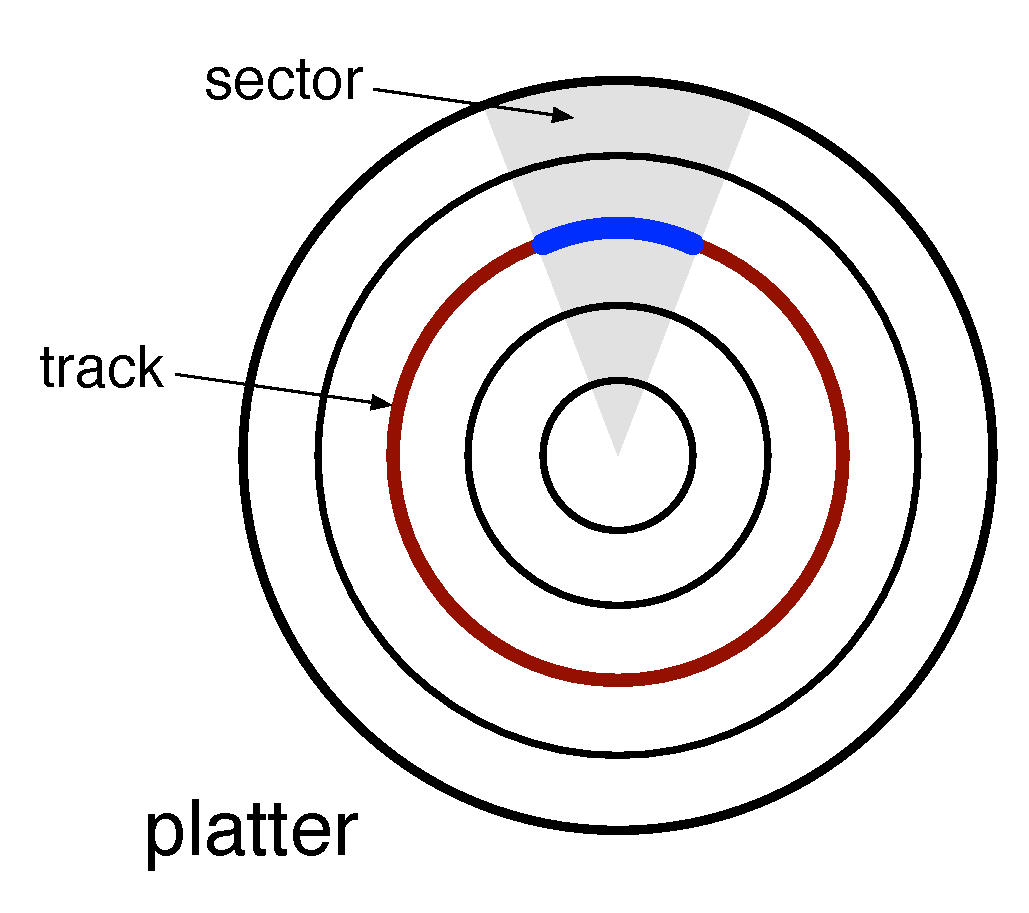
\includegraphics[width=0.7\textwidth]{figures/HDD_sector_track}
\end{column}
\end{columns}
\end{frame}
%
% ---------------------------------------------------------------------------
%
\begin{frame}
\vskip1em
\begin{BOX}{HDD Seek Time}
Time until the actuator arm moves to the desired track.

- \emph{in expectation}: average time to travel between any two tracks;

- \emph{typical}: between 3ms to 13ms

\vskip1em

\textbf{Data locality}: the seek time between \emph{adjacent} tracks is very short.
\end{BOX}

 \vskip0.5em

\begin{BOX}{HDD Rotational delay}
Time until the desired sector arrives under the head.

- \emph{in expectation}: time for a half-rotation of the disk;
\end{BOX}

\vskip1em
\begin{columns}
\begin{column}{0.4\textwidth}
\vskip0.5em
Practice: rotational delay of a 5400rpm disk?
\end{column}
\begin{column}{0.5\textwidth}
\[\frac{0.5 r}{5400 rpm / (60s/m)} = 5.6ms\]
\end{column}
\end{columns}
\end{frame}

%
% ---------------------------------------------------------------------------
%
\begin{frame}{Data transfer between memory and storage}

Data moves between memory and storage in \textbf{fixed-sized} chunks, called \highlight{blocks}.\\
- the block size is a system parameter configured when the device is formatted\\
- the smallest possible block size with a HDD is a single sector;\\
- \emph{typical} sizes are 4KB or 8KB.

\begin{columns}
\begin{column}{0.35\textwidth}
\includegraphics[width=1.1\textwidth]{figures/HDD_architecture}
\end{column}
\begin{column}{0.35\textwidth}
\includegraphics[width=\textwidth]{figures/HDD_block_size}
\end{column}
\end{columns}

In a modern HDD, the controller has an internal, (volatile) DRAM cache, typically of a few MB, which it uses to mediate data transfers with main memory.

\end{frame}

%
% ---------------------------------------------------------------------------
%

\begin{frame}
Solid State Drives (SSDs) have the same architecture as HDDs:

\vskip1em

\includegraphics[width=0.45\textwidth]{figures/HDD_architecture}
~~~
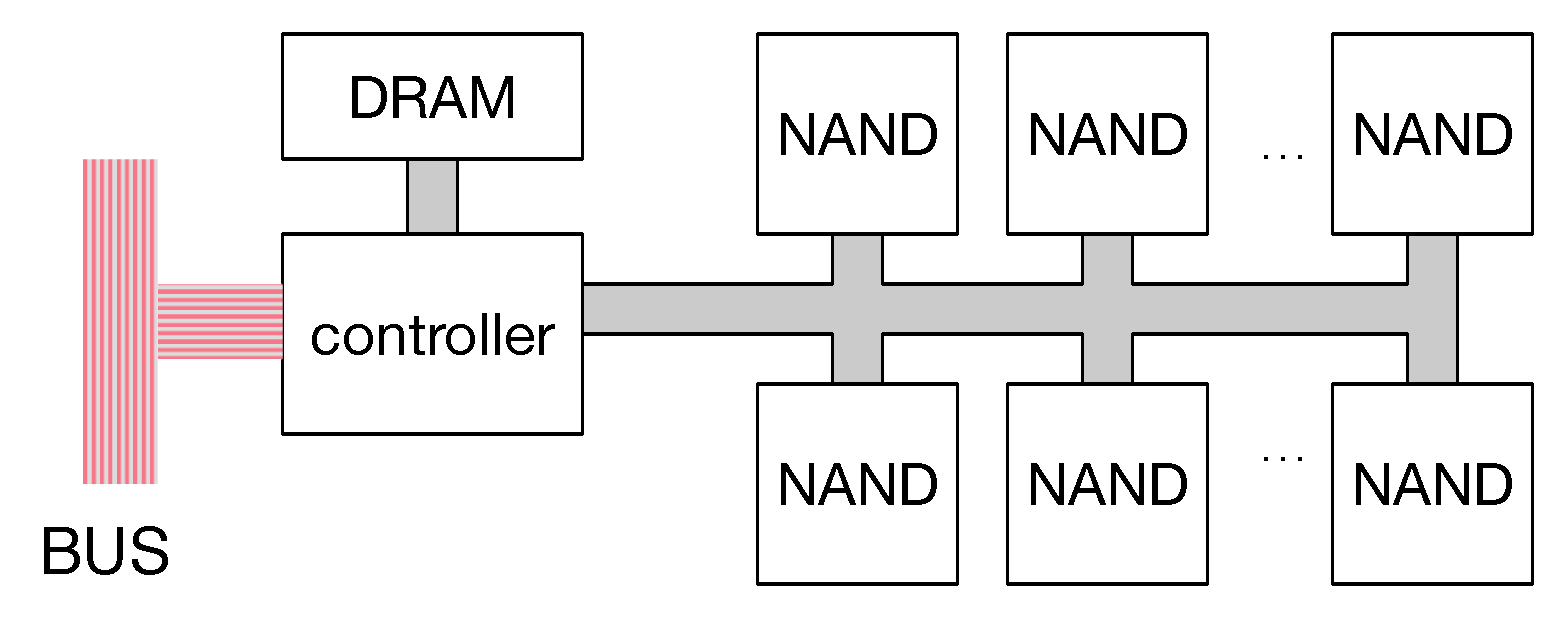
\includegraphics[width=0.45\textwidth]{figures/SSD_architecture}

\vskip1em

Even though they use a much faster medium (NAND) and have no mechanical parts, they are still block-oriented storage devices.
\end{frame}

%
% ---------------------------------------------------------------------------
%
\begin{frame}

RAID (Redundant Arrays of Inexpensive Disks) group multiple disks into a single logical storage device:

\vskip1em

\begin{center}
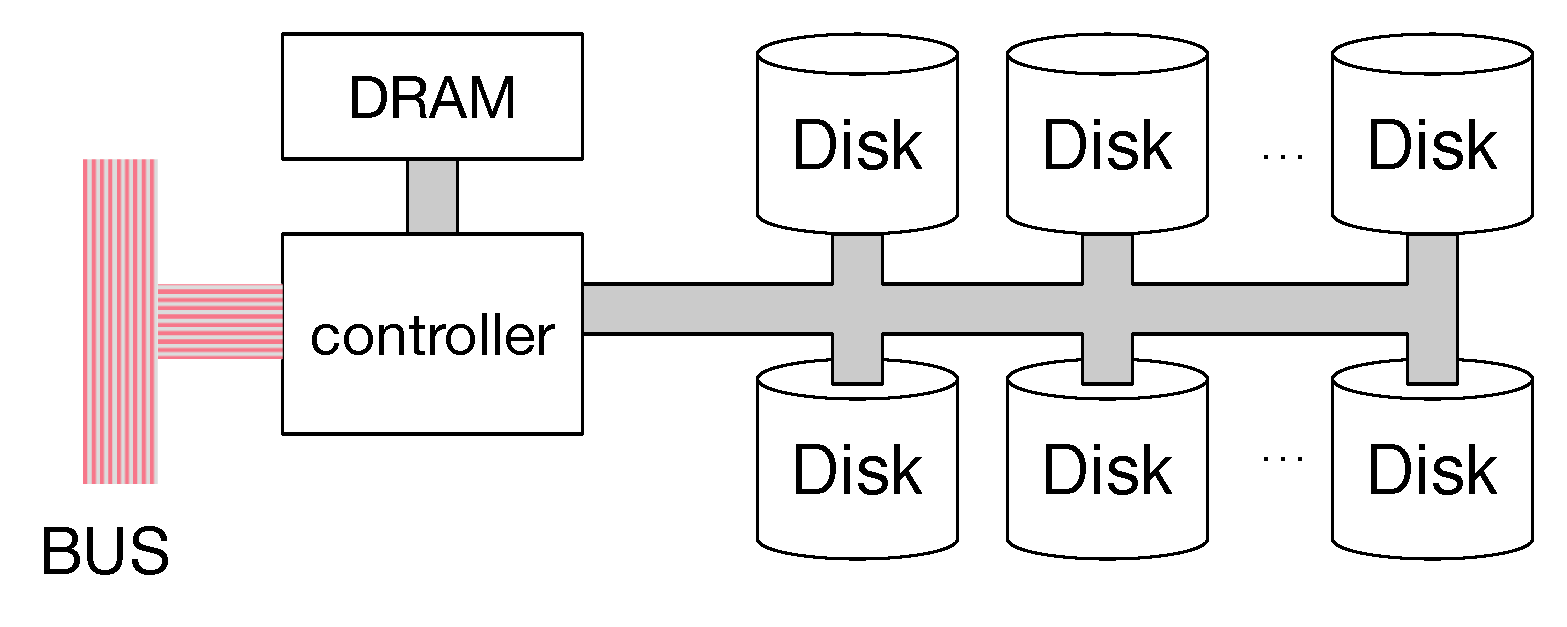
\includegraphics[width=0.45\textwidth]{figures/RAID_architecture}
\end{center}

\vskip1em

Typical RAID settings\footnote{There are many ways of configuring RAID systems.} store the same (logical) block in more than one disk. This yields higher performance and error recovery:
\begin{itemize}[-,topsep=-0.1em]
\item Each block can be read from any disk containing it;\\
\item If one disk crashes, its blocks can be read from another disk.
\end{itemize}
\end{frame}

%
% ---------------------------------------------------------------------------
%
\begin{frame}{Storage is block oriented}
\label{block_oriented_storage}

The Operating System abstracts all storage devices (HDDs, SDDs, RAID arrays, etc.) as a collection of blocks:\\
 - each block has an address;\\
 - file (names) are associated to blocks by the OS

\vskip1em

 \begin{center}
 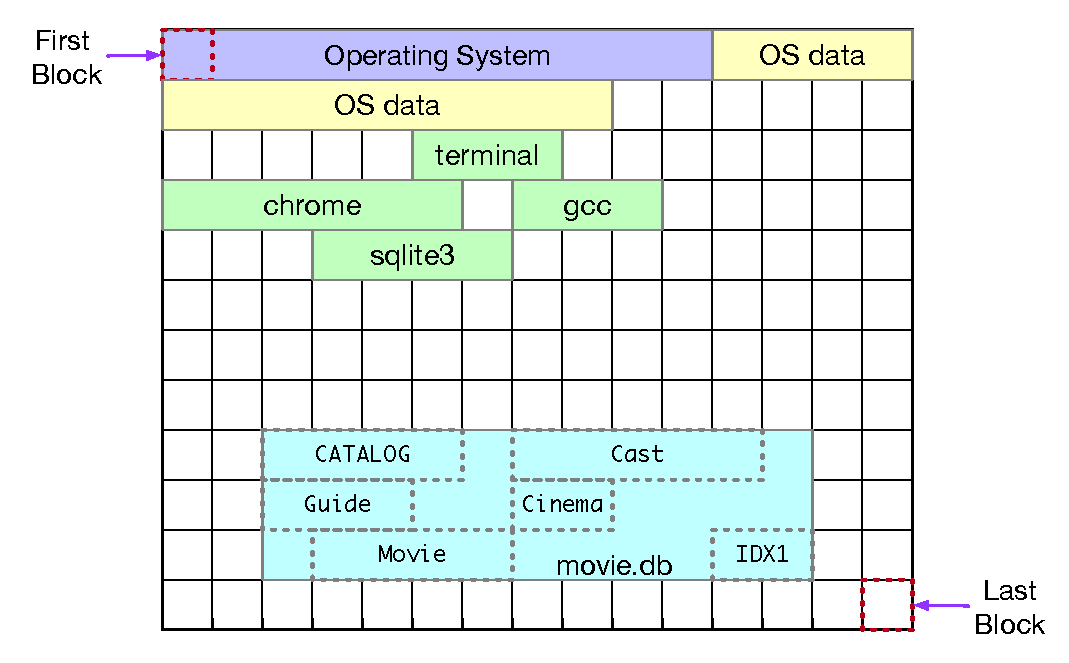
\includegraphics[width=0.75\textwidth]{figures/blocks_on_storage.eps}
 \end{center}

\end{frame}

%
% ---------------------------------------------------------------------------
%



%
% ---------------------------------------------------------------------------
%
\begin{frame}
There are two main costs when using storage:\\
- \textbf{access time}: setting the device to read/write the desired block;\\
- \textbf{transfer time}: moving data between \emph{primary memory} and the device's internal cache.\footnote{The time to move data inside the device is usually ignored.}

\vskip1em

\begin{BOX}{Access times}
- For SSDs and RAID stores, the access time is negligible (and usually very hard to model)\\
- For HDDs, access times are:

\begin{itemize}
\item[\textbf{read}:] average seek time + 0.5 rotational delay
\item[\textbf{write}:] average seek time + 1.5 rotational delay\footnotemark
\end{itemize}
\end{BOX}
\footnotetext{To verify the data was correctly written.}
\end{frame}


%
% ---------------------------------------------------------------------------
%
\begin{frame}{Memory Hierarchy}
\begin{columns}
\begin{column}{0.8\textwidth}

The ``memory'' of a computer is complex and layered sub-system comprising persistent storage, RAM, caches, and registers.

\vskip1em

\begin{BOX}{Cost/Speed}
The closer to the CPU, the faster and more expensive the memory is.
\end{BOX}


\vskip1em

\begin{minipage}{\textwidth}
\footnotesize
\begin{tabular}{l|l|c|c}
\hline
\multirow{2}{*}{\textbf{component}} & \multirow{2}{*}{\textbf{technology}} & \textbf{access} & \textbf{\$/GB} \\
& & \textbf{time (ns)} & \textbf{(2012)}\\
\hline\hline
cache & SRAM & 0.5--2.5 & 500--700\\
\hline
main memory & DRAM & 50--70 & 10--20\\
\hline\hline
\multirow{2}{*}{storage} & flash & 5E3--5E4 & 0.75--1.00 \\
\cline{2-4}
& disk & 5E6 -- 2E7 & 0.05 -- 0.10\\
\hline
\end{tabular}
\vskip1em
\hfill [Patterson \& Hennessy 2014]
\end{minipage}
\end{column}
\begin{column}{0.2\textwidth}
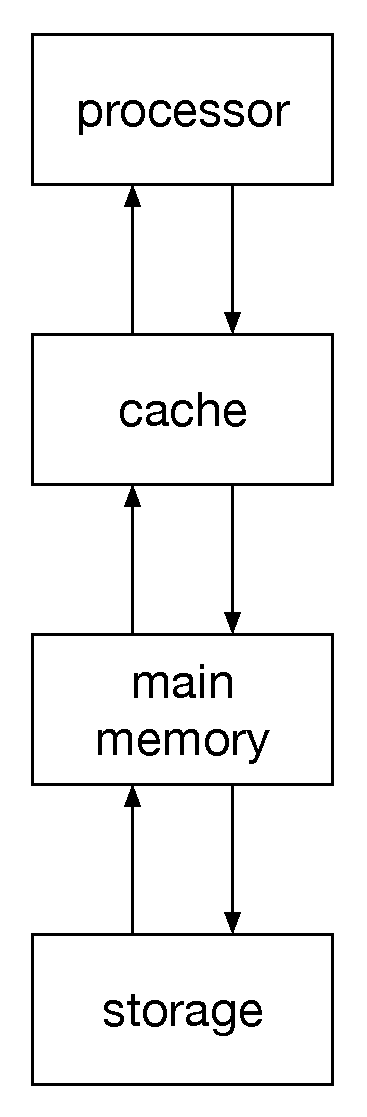
\includegraphics[width=0.8\textwidth]{./figures/memory_hierarchy}
\end{column}
\end{columns}
\end{frame}


%
% ---------------------------------------------------------------------------
%
% \begin{frame}

% \begin{columns}
% \begin{column}{0.8\textwidth}

% When the CPU needs to read a memory cell:\\
% (1) it first checks if the cell is already in the cache;\\
% (2) if not (called a \emph{cache miss}), the cell is requested from main memory

% \vskip1em

% Data comes from memory to the cache in large chunks, to minimize the chance of another cache miss in the very next instruction\footnotemark.

% \vskip2em
% \begin{BOX}{Cache misses waste CPU cycles}
% \textbf{No computation} happens during a cache miss, which must be \emph{avoided} at all costs.
% \end{BOX}

% \end{column}
% \begin{column}{0.2\textwidth}
% 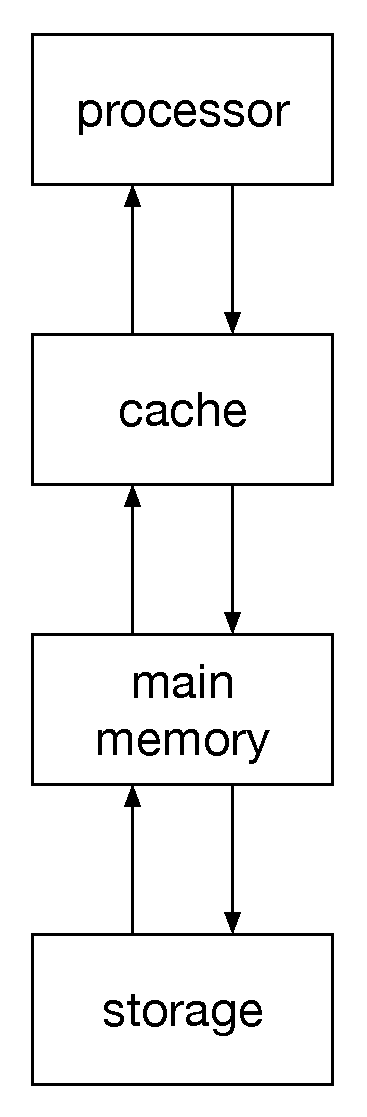
\includegraphics[width=0.8\textwidth]{./figures/memory_hierarchy}
% \end{column}
% \end{columns}

% \footnotetext{The property that a program is likely to use adjacent memory cells in a short period of time is called \emph{locality}.}

% \end{frame}

%
% ---------------------------------------------------------------------------
%
% \begin{frame}

% \begin{columns}
% \begin{column}{0.5\textwidth}
% \textbf{Data Hungry CPUs:}

% How many instructions could a Core i7-3820 execute during the time 4KB of data are transferred from disk to memory?

% \end{column}
% \begin{column}{0.5\textwidth}
% \begin{block}{Intel Core i7-3820 CPU}
% \small
% - 4 processors working at 3.6GHz

% - can theoretically execute up to \(4 \times 3.6 = 14.4\) \textbf{billion} instructions every second

% - it's DMI bus supports up to 2GB/s 
% \end{block}
% \end{column}
% \end{columns}

% \vskip1em

% \begin{BOX}{Program vs CPU instructions}
% Each instruction in a program in a high-level language (e.g., a \lstinline{printf()} statement) gets compiled into many (sometimes thousands) of CPU instructions. Nevertheless, a computer with many fast cores is bound to waste many ``idle'' cycles while data gets transferred from memory.
% \end{BOX}

% \end{frame}
